\begin{figure}[t]
\centering
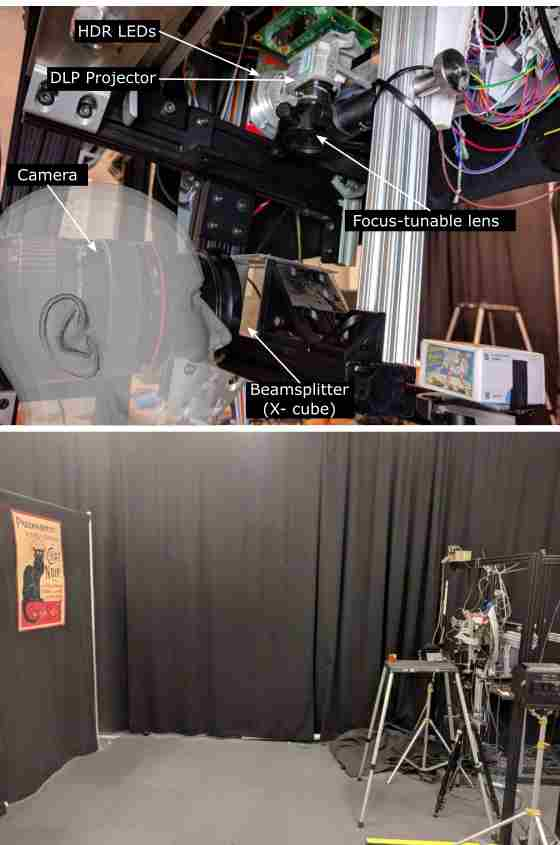
\includegraphics[width=0.8\columnwidth]{images/volumetric/setup}
\caption[Volumetric NED: prototype and staged real-world scene for capturing results]{\emph{Top:} Our prototype display. \emph{Bottom:} The staged real-world scene used to collect all see-through images and videos. Multiple objects (a tiny rubber ducky (2cm height), a wristwatch, a Rubik's cube, and a wall poster) are arranged progressively from near to far. Virtual objects are rendered in this staged real-world scene such that each virtual object is located at the same depth as one of the real world objects (See Figure~\ref{fig:volumetric:results}).}
\label{fig:volumetric:setup}
\end{figure}

